\documentclass[12pt,a4paper]{article}

% ─── Page Layout ───────────────────────────────────────────────────────────────
\usepackage[a4paper, margin=0.8in, headheight=14pt]{geometry}

% ─── Fonts (XeLaTeX) ───────────────────────────────────────────────────────────
\usepackage{fontspec}
\usepackage{unicode-math}
\setmainfont{TeX Gyre Pagella}
\setmonofont[Scale=0.88]{TeX Gyre Cursor}
\setmathfont{Latin Modern Math}

% ─── Packages ──────────────────────────────────────────────────────────────────
\usepackage{xcolor}
\usepackage{colortbl}
\usepackage{titlesec}
\usepackage{enumitem}
\usepackage{tabularx}
\usepackage{booktabs}
\usepackage{array}
\usepackage{amsmath}
\usepackage{tikz}
\usetikzlibrary{shapes.geometric, arrows.meta, positioning, calc, fit, decorations.pathreplacing}
\usepackage{tcolorbox}
\tcbuselibrary{skins, breakable}
\usepackage{hyperref}
\usepackage{fancyhdr}
\usepackage{graphicx}
\usepackage{microtype}
\hyphenpenalty=10000
\exhyphenpenalty=10000
\sloppy
\usepackage{caption}
\usepackage{setspace}
\usepackage{multirow}
\usepackage{tocloft}

% ─── Q&A helper ────────────────────────────────────────────────────────────────
\newcommand{\Q}[1]{\textbf{#1}\par\noindent\ignorespaces}

% ─── Colour Palette ────────────────────────────────────────────────────────────
\definecolor{myred}{RGB}{196,30,58}
\definecolor{mydark}{RGB}{30,30,50}
\definecolor{mygreen}{RGB}{14,120,80}
\definecolor{myteal}{RGB}{0,130,140}
\definecolor{myamber}{RGB}{180,100,0}
\definecolor{mypurple}{RGB}{100,30,160}
\definecolor{mygray}{RGB}{246,247,249}
\definecolor{mgframe}{RGB}{180,185,200}
\definecolor{watermark}{RGB}{145,150,170}
\definecolor{hdrred}{RGB}{250,232,235}
\definecolor{hdrgreen}{RGB}{220,244,233}
\definecolor{hdrteal}{RGB}{220,242,244}
\definecolor{hdramber}{RGB}{253,242,215}
\definecolor{hdrpurple}{RGB}{238,228,255}
\definecolor{hdrgray}{RGB}{238,240,245}
\definecolor{rowalt}{RGB}{250,251,253}

% ─── Section Formatting ────────────────────────────────────────────────────────
\titleformat{\section}
  {\large\bfseries\color{myred}}{\thesection.}{0.5em}{}
  [\vspace{1pt}{\color{myred}\rule{\linewidth}{0.8pt}}]
\titleformat{\subsection}
  {\normalsize\bfseries\color{myteal}}{\thesubsection}{0.5em}{}
\titlespacing*{\section}{0pt}{18pt}{7pt}
\titlespacing*{\subsection}{0pt}{11pt}{4pt}

% ─── Paragraph ─────────────────────────────────────────────────────────────────
\setlength{\parindent}{0pt}
\setlength{\parskip}{4pt}

% ─── TOC Styling ───────────────────────────────────────────────────────────────
\renewcommand{\cfttoctitlefont}{\large\bfseries\color{myred}}
\renewcommand{\cftaftertoctitle}{\par\noindent{\color{myred}\rule{\linewidth}{0.8pt}}}
\setlength{\cftbeforetoctitleskip}{0pt}
\setlength{\cftaftertoctitleskip}{6pt}
\renewcommand{\cftsecfont}{\normalsize\bfseries\color{mydark}}
\renewcommand{\cftsecpagefont}{\normalsize\bfseries\color{mydark}}
\renewcommand{\cftsecleader}{\cftdotfill{\cftdotsep}}
\setlength{\cftbeforesecskip}{7pt}
\renewcommand{\cftsubsecfont}{\small\color{mydark}}
\renewcommand{\cftsubsecpagefont}{\small\color{mydark}}
\setlength{\cftbeforesubsecskip}{3pt}
\setlength{\cftsubsecindent}{1.4em}

% ─── Table helpers ─────────────────────────────────────────────────────────────
\renewcommand{\arraystretch}{1.45}
\setlength{\tabcolsep}{6pt}
\arrayrulecolor{mydark}
\newcolumntype{B}[1]{>{\small\bfseries\raggedright\arraybackslash}m{#1}}
\newcolumntype{Y}{>{\small\raggedright\arraybackslash}X}
\renewcommand{\tabularxcolumn}[1]{m{#1}}

% ─── Header / Footer ───────────────────────────────────────────────────────────
\pagestyle{fancy}
\fancyhf{}
\fancyhead[L]{\small\color{myred}\textbf{OE-EC604C}\;\color{mydark}--- Object Oriented Programming}
\fancyhead[R]{\small\color{myteal}\textbf{Module 5 Notes}}
\fancyfoot[C]{\small\color{mydark}\thepage}
\fancyfoot[R]{\small\color{watermark}\textit{\copyright\ Biraj}}
\renewcommand{\headrulewidth}{0.5pt}
\renewcommand{\footrulewidth}{0.3pt}

% ─── Hyperref ──────────────────────────────────────────────────────────────────
\hypersetup{
  colorlinks=true, linkcolor=myteal, urlcolor=myteal,
  pdfauthor={Biraj Sarkar},
  pdftitle={OE-EC604C --- Module 5 Notes}
}

% ─── tcolorbox styles ──────────────────────────────────────────────────────────
\tcbset{
  tikzbox/.style={
    colback=mygray, colframe=mgframe, boxrule=0.6pt, arc=4pt,
    left=8pt, right=8pt, top=6pt, bottom=6pt,
    colbacktitle=mgframe, coltitle=mydark,
    fonttitle=\small\bfseries
  },
  defbox/.style={
    colback=hdrgreen, colframe=mygreen, boxrule=0.8pt, arc=4pt,
    left=9pt, right=9pt, top=6pt, bottom=6pt,
    colbacktitle=mygreen, coltitle=white,
    fonttitle=\small\bfseries
  },
  formulabox/.style={
    colback=hdrteal, colframe=myteal, boxrule=0.8pt, arc=4pt,
    left=9pt, right=9pt, top=7pt, bottom=7pt,
    colbacktitle=myteal, coltitle=white,
    fonttitle=\small\bfseries
  },
  examplebox/.style={
    colback=hdramber, colframe=myamber, boxrule=0.8pt, arc=4pt,
    left=9pt, right=9pt, top=6pt, bottom=6pt,
    colbacktitle=myamber, coltitle=white,
    fonttitle=\small\bfseries
  },
  masonbox/.style={
    colback=hdrpurple, colframe=mypurple, boxrule=0.8pt, arc=4pt,
    left=9pt, right=9pt, top=6pt, bottom=6pt,
    colbacktitle=mypurple, coltitle=white,
    fonttitle=\small\bfseries
  },
  exambox/.style={
    colback=hdrpurple, colframe=mypurple, boxrule=1pt, arc=5pt,
    left=10pt, right=10pt, top=8pt, bottom=8pt,
    colbacktitle=mypurple, coltitle=white,
    fonttitle=\bfseries,
    breakable, title after break={\textbf{Frequently Asked / Viva Questions (contd.)}}}
}

% XeLaTeX pdfcol fix: reset text color after every tcolorbox
\tcbset{after={\color{black}}}

% ─── TikZ styles ───────────────────────────────────────────────────────────────
\tikzset{
  block/.style={rectangle, draw=myteal, fill=hdrteal,
    text width=2.4cm, align=center, minimum height=0.95cm,
    font=\small, rounded corners=3pt, line width=0.7pt},
  redblock/.style={rectangle, draw=myred, fill=hdrred,
    text width=2.4cm, align=center, minimum height=0.95cm,
    font=\small, rounded corners=3pt, line width=0.7pt},
  netnode/.style={rectangle, draw=myteal, fill=hdrteal,
    text width=1.5cm, align=center, minimum height=0.8cm,
    font=\small, rounded corners=3pt, line width=0.7pt},
  sumjunc/.style={circle, draw=myamber, fill=hdramber,
    minimum size=0.62cm, font=\small, line width=0.8pt},
  snode/.style={circle, draw=mypurple, fill=hdrpurple,
    minimum size=0.55cm, font=\footnotesize, line width=0.7pt},
  arrow/.style={-Stealth, thick, color=mydark},
  redarrow/.style={-Stealth, thick, color=myred},
  line/.style={thick, color=mydark}
}

% ═══════════════════════════════════════════════════════════════════════════════
\begin{document}
% ═══════════════════════════════════════════════════════════════════════════════

\begin{center}
  {\LARGE\bfseries\color{myred} OE-EC604C --- Object Oriented Programming}\\[5pt]
  {\normalsize\color{mydark} Semester VI \quad$\bullet$\quad 3L:0T:0P \quad$\bullet$\quad 3 Credits}\\[3pt]
  {\normalsize\color{myteal}\textbf{Module 5 Exam Notes: Operator Overloading}}\\[3pt]
  {\small\color{mydark} CGEC \;$|$\; B.Tech ECE (2023--27) \;$|$\; \textit{Biraj Sarkar}}
\end{center}
\vspace{2pt}
\noindent{\color{myred}\rule{\linewidth}{1.5pt}}
\vspace{2pt}

\hypersetup{linkcolor=mydark}
\tableofcontents
\hypersetup{linkcolor=myteal}
\newpage

% ===============================================================================
\section{Fundamentals of Operator Overloading}
% ===============================================================================

Operator overloading is a feature of compile-time polymorphism that allows user-defined types (classes) to interact using standard C++ operators.

\subsection{General Rules and Syntax}
When overloading operators in C++, the following rules must be observed:
\begin{itemize}[leftmargin=*, itemsep=3pt]
  \item Only existing operators can be overloaded. New operators (like \texttt{**} or \texttt{<>}) cannot be created.
  \item The precedence and associativity of operators remain unchanged.
  \item Overloaded operators must have at least one operand of user-defined type (class/enum).
  \item Original syntax templates (e.g., number of operands) must be maintained.
\end{itemize}

\begin{tcolorbox}[defbox, title={\textbf{List of Operators that Cannot be Overloaded}}]
The following operators are strictly restricted from being overloaded:
\begin{enumerate}[label=\textbf{\arabic*.}, leftmargin=2em, itemsep=1pt]
  \item Class member access operator (\texttt{.})
  \item Pointer-to-member operator (\texttt{.*})
  \item Scope resolution operator (\texttt{::})
  \item Ternary conditional operator (\texttt{?:})
  \item Sizeof operator (\texttt{sizeof})
\end{enumerate}
\end{tcolorbox}

\begin{tcolorbox}[formulabox, title={\textbf{Operator Overloading Signature Syntax}}]
\begin{align}
  &\text{As Member Function: } && \text{Return\_Type} \quad \text{operator}\;\text{OP}\;(\text{Arguments}) \quad \{ \dots \} \\
  &\text{As Friend Function: } && \texttt{friend} \quad \text{Return\_Type} \quad \text{operator}\;\text{OP}\;(\text{Arguments}) \quad \{ \dots \}
\end{align}
\end{tcolorbox}

% ===============================================================================
\section{Binary \& Unary Operator Overloading}
% ===============================================================================

Operators are overloaded differently based on whether they are unary (one operand) or binary (two operands), and whether member or friend functions are used.

\subsection{Unary Operator Overloading}
Unary operators operate on a single operand.
\begin{itemize}[leftmargin=*, itemsep=3pt]
  \item \textbf{Member Function implementation:} Takes \textbf{zero} arguments (the operand is implicitly passed via the \texttt{this} pointer).
  \item \textbf{Friend Function implementation:} Takes \textbf{one} argument explicitly.
  \item \textbf{Increment/Decrement Ambiguity:} To distinguish between prefix (e.g., \texttt{++obj}) and postfix (e.g., \texttt{obj++}), C++ uses a dummy \texttt{int} parameter in the postfix signature.
\end{itemize}

\begin{tcolorbox}[examplebox, title={Code Example: Prefix and Postfix operator overloading}]
\begin{spacing}{1.0}
\begin{verbatim}
#include <iostream>
class Counter {
private:
    int value;
public:
    Counter(int v = 0) : value(v) {}
    
    // Prefix ++ (e.g., ++c)
    Counter operator++() {
        ++value;
        return *this; // Returns incremented object
    }
    
    // Postfix ++ (e.g., c++) -> Note the dummy 'int' parameter
    Counter operator++(int) {
        Counter temp = *this; // Save original state
        value++; // Increment
        return temp; // Return original state
    }
    
    int getValue() { return value; }
};
\end{verbatim}
\end{spacing}
\end{tcolorbox}

\subsection{Binary Operator Overloading}
Binary operators operate on two operands (e.g., \texttt{a + b}).
\begin{itemize}[leftmargin=*, itemsep=3pt]
  \item \textbf{Member Function implementation:} Takes \textbf{one} argument explicitly. The left-hand operand is the calling object, and the right-hand operand is passed as the argument.
  \item \textbf{Friend Function implementation:} Takes \textbf{two} arguments explicitly.
\end{itemize}

\begin{tcolorbox}[examplebox, title={Code Example: Relational operator overloading for custom strings}]
\begin{spacing}{1.0}
\begin{verbatim}
#include <iostream>
#include <cstring>
class String {
private:
    char *str;
public:
    String(const char *s) {
        str = new char[strlen(s) + 1];
        strcpy(str, s);
    }
    ~String() { delete[] str; }
    
    // Overload == operator
    bool operator==(const String &s) {
        return strcmp(str, s.str) == 0;
    }
    
    // Overload < operator
    bool operator<(const String &s) {
        return strcmp(str, s.str) < 0;
    }
};
\end{verbatim}
\end{spacing}
\end{tcolorbox}

\subsection{Stream Insertion (\texttt{<<}) and Extraction (\texttt{>>}) Overloading}
Stream operators must be overloaded as \textbf{friend functions} because the left-hand operand is a stream object (like \texttt{std::ostream}), not an instance of our class.

\begin{tcolorbox}[tikzbox, title={Stream I/O Data Flow Block Diagram}]
\centering
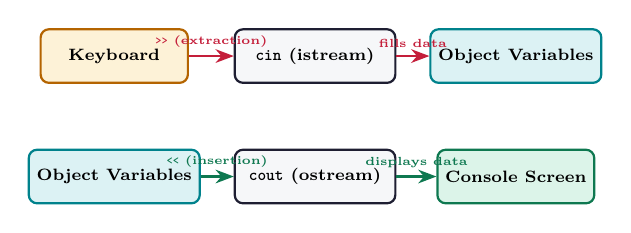
\begin{tikzpicture}[node distance=1.5cm, thick, scale=0.85, every node/.style={scale=0.85}]
  % Input Stream Flow
  \node[rectangle, draw=myamber, fill=hdramber, rounded corners=3pt, minimum width=2.2cm, minimum height=0.8cm, font=\scriptsize\bfseries] (keyboard) at (-3.5, 0.8) {Keyboard};
  \node[rectangle, draw=mydark, fill=mygray, rounded corners=3pt, minimum width=2.4cm, minimum height=0.8cm, font=\scriptsize\bfseries] (istream) at (-0.5, 0.8) {\texttt{cin} (istream)};
  \node[rectangle, draw=myteal, fill=hdrteal, rounded corners=3pt, minimum width=2.2cm, minimum height=0.8cm, font=\scriptsize\bfseries] (objIn) at (2.5, 0.8) {Object Variables};

  \draw[arrow, color=myred] (keyboard) -- (istream) node[midway, above, font=\tiny\bfseries] {\texttt{>>} (extraction)};
  \draw[arrow, color=myred] (istream) -- (objIn) node[midway, above, font=\tiny\bfseries] {fills data};

  % Output Stream Flow
  \node[rectangle, draw=myteal, fill=hdrteal, rounded corners=3pt, minimum width=2.2cm, minimum height=0.8cm, font=\scriptsize\bfseries] (objOut) at (-3.5, -1.0) {Object Variables};
  \node[rectangle, draw=mydark, fill=mygray, rounded corners=3pt, minimum width=2.4cm, minimum height=0.8cm, font=\scriptsize\bfseries] (ostream) at (-0.5, -1.0) {\texttt{cout} (ostream)};
  \node[rectangle, draw=mygreen, fill=hdrgreen, rounded corners=3pt, minimum width=2.2cm, minimum height=0.8cm, font=\scriptsize\bfseries] (console) at (2.5, -1.0) {Console Screen};

  \draw[arrow, color=mygreen] (objOut) -- (ostream) node[midway, above, font=\tiny\bfseries] {\texttt{<<} (insertion)};
  \draw[arrow, color=mygreen] (ostream) -- (console) node[midway, above, font=\tiny\bfseries] {displays data};
\end{tikzpicture}
\end{tcolorbox}

% ===============================================================================
\section{Type Conversions}
% ===============================================================================

C++ allows custom type conversions between primitive types and class objects.

\subsection{Basic Type to Class Type}
Handled automatically using a \textbf{parameterized constructor} inside the target class that accepts the basic type as an argument.
\begin{equation}
  \texttt{Time t1 = 95; // Invokes constructor Time(int) to convert minutes}
\end{equation}

\subsection{Class Type to Basic Type}
Accomplished by defining a \textbf{casting operator function} (conversion function) inside the class.
\textbf{Rules for Conversion Functions:}
\begin{itemize}[leftmargin=*, itemsep=2pt]
  \item It must be a class member function.
  \item It must not specify any return type (the return type is implicit from the operator's name).
  \item It must not accept any arguments.
\end{itemize}
\begin{equation}
  \text{Syntax: } \quad \texttt{operator}\;\text{Basic\_Type}\;() \quad \{ \quad \text{return}\;\text{value}; \quad \}
\end{equation}

\begin{tcolorbox}[examplebox, title={Code Example: Basic-to-Class and Class-to-Basic conversions}]
\begin{spacing}{1.0}
\begin{verbatim}
#include <iostream>
class Time {
private:
    int hours, minutes;
public:
    Time() : hours(0), minutes(0) {}
    
    // Basic to Class Conversion (Constructor)
    Time(int mins) {
        hours = mins / 60;
        minutes = mins % 60;
    }
    
    // Class to Basic Conversion (Casting Operator)
    operator int() {
        return (hours * 60) + minutes;
    }
    
    void display() {
        std::cout << hours << "h " << minutes << "m" << std::endl;
    }
};

int main() {
    // Basic -> Class
    Time t1 = 85; // Converts 85 (int) to 1h 25m (Time)
    t1.display(); // Prints: 1h 25m

    // Class -> Basic
    int totalMins = t1; // Converts Time to int using operator int()
    std::cout << "Total minutes = " << totalMins << std::endl; // 85
    return 0;
}
\end{verbatim}
\end{spacing}
\end{tcolorbox}

% ===============================================================================
% MANDATORY QUICK REVISION PAGE
% ===============================================================================
\newpage
\begin{center}
  {\large\bfseries\color{myred} Quick Revision --- Module V}\\[3pt]
  {\small\color{mydark} Operator Overloading $|$ OE-EC604C}
\end{center}
\noindent{\color{myred}\rule{\linewidth}{1.2pt}}
\vspace{4pt}

\begin{tcolorbox}[formulabox, title={\textbf{Key Overloading Signatures}}]
\renewcommand{\arraystretch}{1.3}
\begin{tabularx}{\linewidth}{B{3.8cm} X}
Unary (Member)           & \texttt{Counter operator++() \{ /* prefix */ \}} \\[4pt]
Unary Postfix (Member)   & \texttt{Counter operator++(int) \{ /* dummy int parameter */ \}} \\[4pt]
Binary (Member)          & \texttt{Complex operator+(const Complex \&c) \{ /* 1 arg */ \}} \\[4pt]
Binary (Friend)          & \texttt{friend Complex operator+(Complex \&c1, Complex \&c2); // 2 args} \\[4pt]
Stream Insertion         & \texttt{friend ostream\& operator<<(ostream\& out, const MyClass \&obj);} \\[4pt]
Casting Function         & \texttt{operator float() \{ return data; \} // No return type specified}
\end{tabularx}
\end{tcolorbox}

\begin{tcolorbox}[defbox, title={\textbf{One-Line Definitions}}]
\begin{itemize}[leftmargin=*, itemsep=2.5pt, topsep=0pt]
  \item \textbf{Operator Overloading:} Assigning new functionalities to C++ operators when applied to class instances.
  \item \textbf{Stream Extraction (>>):} An overloaded operator used to extract formatted values from an input stream.
  \item \textbf{Stream Insertion (<<):} An overloaded operator used to insert formatted values into an output stream.
  \item \textbf{Conversion Operator:} A special class member function used to convert an object into another data type.
  \item \textbf{Prefix Operator:} An increment or decrement operator executed before evaluation of the expression.
  \item \textbf{Postfix Operator:} An increment or decrement operator executed after evaluation of the expression.
  \item \textbf{Basic to Class Conversion:} Converting standard types to user classes via parameterized constructors.
  \item \textbf{Class to Basic Conversion:} Converting classes to standard types via overloaded casting operators.
  \item \textbf{This Pointer:} An implicit pointer inside member functions that points to the calling object instance.
\end{itemize}
\end{tcolorbox}

\begin{tcolorbox}[exambox, title={\textbf{Frequently Asked / Viva Questions}}]
\begin{enumerate}[topsep=0pt, label=\textbf{Q\arabic*.}, itemsep=5pt]
  \item \Q{Which operators cannot be overloaded in C++? Why?}
    Operators like \texttt{.}, \texttt{.*}, \texttt{::}, \texttt{?:}, and \texttt{sizeof} cannot be overloaded to protect C++ syntax structures and core language bindings from corruption.
  \item \Q{Why does a postfix overloaded operator require a dummy \texttt{int} parameter?}
    The compiler uses the \texttt{int} parameter strictly as a signature flag to distinguish postfix calls (\texttt{obj++}) from prefix calls (\texttt{++obj}).
  \item \Q{Why must stream insertion (\texttt{<<}) and extraction (\texttt{>>}) operators be overloaded as friend functions?}
    The left-hand operand is \texttt{ostream} or \texttt{istream}, not our class object. Member functions require the left operand to be the class itself, so a friend function is mandatory.
  \item \Q{What is the difference in arguments between member and friend function operator overloading?}
    For binary operators: member functions take 1 argument (left operand is implicit); friend functions take 2 arguments explicitly. For unary operators: member functions take 0 arguments; friend functions take 1.
  \item \Q{Can we change the basic behaviors of operators (like changing $+$ to subtract)?}
    Yes, syntactically possible, but highly discouraged as it violates design clarity and makes code unreadable.
  \item \Q{What are the restrictions on type conversion functions?}
    They must be non-static class member functions, cannot have arguments, and must not specify a return type.
  \item \Q{Explain conversion from one class type to another class type.}
    This can be done using: (1) A constructor in the destination class that accepts the source class, or (2) A casting operator inside the source class that returns the destination class.
  \item \Q{Can we overload the assignment operator (\texttt{=}) as a friend function?}
    No. C++ rules mandate that \texttt{=}, \texttt{()}, \texttt{[]}, and \texttt{->} must be overloaded \textit{only} as member functions to prevent compiler syntax conflicts.
  \item \Q{What is the return type of stream insertion (\texttt{<<}) and extraction (\texttt{>>}) operators?}
    They return a reference to the stream object (\texttt{ostream\&} or \texttt{istream\&}). This allows chaining (e.g., \texttt{cout << a << b;}).
  \item \Q{Does operator overloading change the execution speed of a program?}
    No. Operator overloading is resolved at compile time (static binding), so it has zero runtime overhead compared to equivalent function calls.
  \item \Q{Is it possible to overload operators for standard types (like overloading $+$ for two integers)?}
    No. At least one operand must be a user-defined class or structure to prevent overriding standard arithmetic logic.
  \item \Q{Can we use default arguments in overloaded operators?}
    No, default arguments are not permitted in overloaded operators because they could conflict with the operator's expected arity.
\end{enumerate}
\end{tcolorbox}

\begin{tcolorbox}[tikzbox, title={Comparison: Member Functions vs. Friend Functions for Overloading}]
\renewcommand{\arraystretch}{1.45}
\par\noindent
\begin{tabularx}{\linewidth}{|B{3.2cm}|Y|Y|}
\hline
\textbf{Feature} & \textbf{\color{myteal}Member Function Overloading} & \textbf{\color{myamber}Friend Function Overloading} \\
\hline
\textbf{Implicit Operand} & Passes the left-hand operand implicitly via the \texttt{this} pointer. & No implicit operand. All operands must be explicitly declared in arguments. \\
\hline
\textbf{Left Operand Rule} & Left operand must strictly be an object of the defining class. & Left operand can be of any type (e.g., stream, primitive, other class). \\
\hline
\textbf{Number of Arguments} & Binary: 1 argument; Unary: 0 arguments. & Binary: 2 arguments; Unary: 1 argument. \\
\hline
\textbf{Class Encapsulation} & Maintains strict encapsulation boundaries. & Grants external function access (minor encapsulation bypass). \\
\hline
\textbf{Special Operators} & Mandatory for operators: \texttt{=}, \texttt{[]}, \texttt{()}, \texttt{->}. & Not allowed for: \texttt{=}, \texttt{[]}, \texttt{()}, \texttt{->}. \\
\hline
\end{tabularx}
\end{tcolorbox}

\end{document}
